%% BioMed_Central_Tex_Template_v1.06
%%                                      %
%  bmc_article.tex            ver: 1.06 %
%                                       %

%%IMPORTANT: do not delete the first line of this template
%%It must be present to enable the BMC Submission system to
%%recognise this template!!

%%%%%%%%%%%%%%%%%%%%%%%%%%%%%%%%%%%%%%%%%
%%                                     %%
%%  LaTeX template for BioMed Central  %%
%%     journal article submissions     %%
%%                                     %%
%%          <8 June 2012>              %%
%%                                     %%
%%                                     %%
%%%%%%%%%%%%%%%%%%%%%%%%%%%%%%%%%%%%%%%%%


%%%%%%%%%%%%%%%%%%%%%%%%%%%%%%%%%%%%%%%%%%%%%%%%%%%%%%%%%%%%%%%%%%%%%
%%                                                                 %%
%% For instructions on how to fill out this Tex template           %%
%% document please refer to Readme.html and the instructions for   %%
%% authors page on the biomed central website                      %%
%% http://www.biomedcentral.com/info/authors/                      %%
%%                                                                 %%
%% Please do not use \input{...} to include other tex files.       %%
%% Submit your LaTeX manuscript as one .tex document.              %%
%%                                                                 %%
%% All additional figures and files should be attached             %%
%% separately and not embedded in the \TeX\ document itself.       %%
%%                                                                 %%
%% BioMed Central currently use the MikTex distribution of         %%
%% TeX for Windows) of TeX and LaTeX.  This is available from      %%
%% http://www.miktex.org                                           %%
%%                                                                 %%
%%%%%%%%%%%%%%%%%%%%%%%%%%%%%%%%%%%%%%%%%%%%%%%%%%%%%%%%%%%%%%%%%%%%%

%%% additional documentclass options:
%  [doublespacing]
%  [linenumbers]   - put the line numbers on margins
%  [twocolumn]

\documentclass[twocolumn]{bmcart}

%%% Load packages
%\usepackage{amsthm,amsmath}
%\RequirePackage{natbib}
%\RequirePackage{hyperref}
\usepackage[utf8]{inputenc} %unicode support
%\usepackage{graphicx}
\usepackage{rotating}
%\usepackage[applemac]{inputenc} %applemac support if unicode package fails
%\usepackage[latin1]{inputenc} %UNIX support if unicode package fails


%%%%%%%%%%%%%%%%%%%%%%%%%%%%%%%%%%%%%%%%%%%%%%%%%
%%                                             %%
%%  If you wish to display your graphics for   %%
%%  your own use using includegraphic or       %%
%%  includegraphics, then comment out the      %%
%%  following two lines of code.               %%
%%  NB: These line *must* be included when     %%
%%  submitting to BMC.                         %%
%%  All figure files must be submitted as      %%
%%  separate graphics through the BMC          %%
%%  submission process, not included in the    %%
%%  submitted article.                         %%
%%                                             %%
%%%%%%%%%%%%%%%%%%%%%%%%%%%%%%%%%%%%%%%%%%%%%%%%%


%\def\includegraphic{}
%\def\includegraphics{}



%%% Put your definitions there:
\startlocaldefs
\endlocaldefs


%%% Begin ...
\begin{document}

%%% Start of article front matter
\begin{frontmatter}

\begin{fmbox}
\dochead{Research}

%%%%%%%%%%%%%%%%%%%%%%%%%%%%%%%%%%%%%%%%%%%%%%
%%                                          %%
%% Enter the title of your article here     %%
%%                                          %%
%%%%%%%%%%%%%%%%%%%%%%%%%%%%%%%%%%%%%%%%%%%%%%

\title{Correcting docking pose generation error on binding affinity prediction}

%%%%%%%%%%%%%%%%%%%%%%%%%%%%%%%%%%%%%%%%%%%%%%
%%                                          %%
%% Enter the authors here                   %%
%%                                          %%
%% Specify information, if available,       %%
%% in the form:                             %%
%%   <key>={<id1>,<id2>}                    %%
%%   <key>=                                 %%
%% Comment or delete the keys which are     %%
%% not used. Repeat \author command as much %%
%% as required.                             %%
%%                                          %%
%%%%%%%%%%%%%%%%%%%%%%%%%%%%%%%%%%%%%%%%%%%%%%

\author[
   addressref={aff1},                   % id's of addresses, e.g. {aff1,aff2}
%   corref={aff1},                       % id of corresponding address, if any
%   noteref={n1},                       % id's of article notes, if any
   email={jackyleehongjian@gmail.com}   % email address
]{\inits{HL}\fnm{Hongjian} \snm{Li}}
\author[
   addressref={aff1},                   % id's of addresses, e.g. {aff1,aff2}
   email={ksleung@cse.cuhk.edu.hk}
]{\inits{KSL}\fnm{Kwong-Sak} \snm{Leung}}
\author[
   addressref={aff1},                   % id's of addresses, e.g. {aff1,aff2}
   email={mhwong@cse.cuhk.edu.hk}
]{\inits{MHW}\fnm{Man-Hon} \snm{Wong}}
\author[
   addressref={aff2},
   corref={aff2},                      % id of corresponding address, if any
   email={pedro.ballester@inserm.fr}
]{\inits{PJB}\fnm{Pedro J.} \snm{Ballester}}

%%%%%%%%%%%%%%%%%%%%%%%%%%%%%%%%%%%%%%%%%%%%%%
%%                                          %%
%% Enter the authors' addresses here        %%
%%                                          %%
%% Repeat \address commands as much as      %%
%% required.                                %%
%%                                          %%
%%%%%%%%%%%%%%%%%%%%%%%%%%%%%%%%%%%%%%%%%%%%%%

\address[id=aff1]{
  \orgname{Department of Computer Science and Engineering, Chinese University of Hong Kong},
  \city{Hong Kong},
  \cny{China}
}
\address[id=aff2]{
  \orgname{Cancer Research Center of Marseille, INSERM U1068},
  \street{27 Boulevard Lei Roure},
  \postcode{F-13009}
  \city{Marseille},
  \cny{France}
}

%%%%%%%%%%%%%%%%%%%%%%%%%%%%%%%%%%%%%%%%%%%%%%
%%                                          %%
%% Enter short notes here                   %%
%%                                          %%
%% Short notes will be after addresses      %%
%% on first page.                           %%
%%                                          %%
%%%%%%%%%%%%%%%%%%%%%%%%%%%%%%%%%%%%%%%%%%%%%%

\begin{artnotes}
%\note{Sample of title note}     % note to the article
%\note[id=n1]{Equal contributor} % note, connected to author
\end{artnotes}

%\end{fmbox}% comment this for two column layout

%%%%%%%%%%%%%%%%%%%%%%%%%%%%%%%%%%%%%%%%%%%%%%
%%                                          %%
%% The Abstract begins here                 %%
%%                                          %%
%% Please refer to the Instructions for     %%
%% authors on http://www.biomedcentral.com  %%
%% and include the section headings         %%
%% accordingly for your article type.       %%
%%                                          %%
%%%%%%%%%%%%%%%%%%%%%%%%%%%%%%%%%%%%%%%%%%%%%%

\begin{abstractbox}

\begin{abstract}

\parttitle{Background}
Pose generation error is usually measured by comparing the geometry of the pose generated by the docking software and that of the same molecule co-crystallised with the considered protein. Surprisingly, the impact of this error on binding affinity prediction is yet to be systematically analysed across diverse protein-ligand complexes.

\parttitle{Results}
Against commonly-held views, pose generation error has generally a small impact on the accuracy in binding affinity prediction. This is also true for large pose generation errors and it is not only observed with machine-learning scoring functions, but also with classical scoring functions such as AutoDock Vina. Furthermore, we propose a procedure to correct for this error which consists of calibrating the scoring functions with re-docked, rather than co-crystallised, poses. As a result, test set performance after this error-correcting procedure is virtually the same as that of predicting the binding affinity in the absence of pose generation error (i.e. on crystal structures). We evaluated several strategies, obtaining better results for those using a single docking pose per ligand.

\parttitle{Conclusions}
In practice, binding affinity prediction is carried out on the docking pose of a known binder rather than its co-crystallised pose. Our results suggest than pose generation error is in general far less damaging for binding affinity prediction than it is believed. From a practical stand-point, the proposed procedure does largely correct for this error. The resulting machine learning scoring function is freely-available here.

\end{abstract}

%%%%%%%%%%%%%%%%%%%%%%%%%%%%%%%%%%%%%%%%%%%%%%
%%                                          %%
%% The keywords begin here                  %%
%%                                          %%
%% Put each keyword in separate \kwd{}.     %%
%%                                          %%
%%%%%%%%%%%%%%%%%%%%%%%%%%%%%%%%%%%%%%%%%%%%%%

\begin{keyword}
\kwd{molecular docking}
\kwd{binding affinity}
\kwd{drug discovery}
\kwd{machine learning}
\end{keyword}

% MSC classifications codes, if any
%\begin{keyword}[class=AMS]
%\kwd[Primary ]{}
%\kwd{}
%\kwd[; secondary ]{}
%\end{keyword}

\end{abstractbox}
%
\end{fmbox}% uncomment this for twcolumn layout

\end{frontmatter}

%%%%%%%%%%%%%%%%%%%%%%%%%%%%%%%%%%%%%%%%%%%%%%
%%                                          %%
%% The Main Body begins here                %%
%%                                          %%
%% Please refer to the instructions for     %%
%% authors on:                              %%
%% http://www.biomedcentral.com/info/authors%%
%% and include the section headings         %%
%% accordingly for your article type.       %%
%%                                          %%
%% See the Results and Discussion section   %%
%% for details on how to create sub-sections%%
%%                                          %%
%% use \cite{...} to cite references        %%
%%  \cite{koon} and                         %%
%%  \cite{oreg,khar,zvai,xjon,schn,pond}    %%
%%  \nocite{smith,marg,hunn,advi,koha,mouse}%%
%%                                          %%
%%%%%%%%%%%%%%%%%%%%%%%%%%%%%%%%%%%%%%%%%%%%%%

%%%%%%%%%%%%%%%%%%%%%%%%% start of article main body
% <put your article body there>

%%%%%%%%%%%%%%%%
%% Background %%
%%
\section*{Introduction}

An introduction referencing all our previous papers: concise but comprehensive. You can reuse parts of different papers (e.g. the conclusions to explain the contents of that study).

Fig. 1. Example of pose generation error. Top: crystal structure of the MRV ligand bound to the CCR5 Chemokine Receptor (PDB 4MBS). Bottom: re-docked pose of MRV. Hydrogen bonds are pictured as discontinued lines. The Root-Mean Square Deviation (RMSD) between the co-crystallized and the re-docked poses is 2.1 Å, which quantifies pose generation error. The plots were generated with iview [1], an interactive WebGL visualizer freely available at http://istar.cse.cuhk.edu.hk/iview/ (iview requires no Java plugins, yet supports macromolecular surface construction and virtual reality effects). [this figure but with another ligand to avoid repetition]

\section*{Methods}

Preamble

\subsection*{Multiple Linear Regression (MLR) with Cyscore features}

Model 1 – AutoDock Vina
The AutoDock series [2][3][4] is arguably the most widely used docking software by the research community. AutoDock Vina significantly improved [2] the average accuracy of the binding mode predictions offered by AutoDock 4 [4], while running two orders of magnitude faster with multithreading. Vina was an exciting development, not only due to its remarkable pose generation performance, both in terms of effectiveness and efficiency, but also because it is an open source tool that aids docking method development. 
Vina’s score for the kth pose of a molecule is given by the estimated free energy of binding to the target protein and calculated in Vina as:

	                                               

where
 
 
 

e1 is the predicted free energy of binding reported by Vina when re-scoring the structure of a protein-ligand complex. As usual, to compare to binding affinities (pKd or pKi), the predicted free energy of binding in kcal/mol units is converted into pKd with pKd=-0.73349480509e1 (see for instance [5] for an explanation of how this conversion factor is derived). The values for these weights were found by minimising the difference between predicted and measured binding affinity using a nonlinear optimisation algorithm (this process was not detailed in the original publication [2]).  Further details on each of these Vina terms can be found in [5], including the expressions for intermolecular and intramolecular energetic terms (respectively distinguished with ‘r’ and ‘a’ subscripts above). 
Model 2 – MLR::Vina
In studies based on structural data, there is only one 3D geometry or pose of the molecule (k=1), the co-crystallized ligand, and thus the intramolecular contributions in equation 1 cancel out. This means that, once a co-crystallized ligand is redocked, each of the resulting poses is described by 11 Vina terms. Here, a MLR model, effectively a classical scoring function, is built using the 11 unweighted Vina terms as features. In order to make the problem amenable to MLR, we made a grid search on the w6 weight and thereafter run MLR on the remaining weights as explained in the next section.
Model 3 – RF::Vina
While Vina’s ability to predict binding affinity is among the best provided by classical scoring functions, it is still limited by the assumption of additivity in its functional form. Random Forest (RF) [6] can be used to circumvent modeling assumptions. We therefore built a RF model with the 11 Vina features using the default number of trees (500). Instead of using all features, RF selects the best split at each node of the tree from a typically small number (mtry) of randomly chosen features. The mtry value with the lowest RMSE on Out-of-Bag (OOB) data is selected. 
Model 4 – RF::VinaElem
This is essentially model 3 using a total of 47 features: the 36 RF-Score features [7] in addition to the 11 Vina features. Therefore, for a given random seed, a RF for each mtry value from 1 to 47 is built and that with the lowest RMSE on OOB data is selected as the scoring function. RF-Score features are elemental occurrence counts of a set of protein-ligand atom pairs in a complex. To calculate these features, atom types are selected so as to generate features that are as dense as possible, while considering all the heavy atoms commonly observed in PDB complexes (C, N, O, F, P, S, Cl, Br, I). As the number of protein-ligand contacts is constant for a particular complex, the more atom types are considered the sparser the resulting features will be. Therefore, a minimal set of atom types is selected by considering atomic number only. Furthermore, a smaller set of interaction features has the additional advantage of leading to computationally faster scoring functions. In this way, the features are defined as the occurrence count of intermolecular contacts between elemental atom types i and j:
 
where dkl is the Euclidean distance between the kth protein atom of type j and the lth ligand atom of type i calculated from a structure; Kj is the total number of protein atoms of type j and Li is the total number of ligand atoms of type i in the considered complex;  is the Heaviside step function that counts contacts within a dcutoff neighbourhood. For example, x7,8 is the number of occurrences of protein nitrogen atoms hypothetically interacting with ligand oxygen atoms within a chosen neighbourhood. This representation led to a total of 81 features, of which 45 are zero due to the lack of proteinogenic amino acids with F, P, Cl, Br and I atoms. Therefore, each complex was characterized by a vector with 36 integer-valued features.

\begin{equation}
RMSE = \sqrt{\frac{1}{N}\sum_{n=1}^N(p^{(n)}-y^{(n)})^2}
\label{eqn:rmse}
\end{equation}

\begin{equation}
SD = \sqrt{\frac{1}{N-2}\sum_{n=1}^N(\hat{p}^{(n)}-y^{(n)})^2}
\label{eqn:sdev}
\end{equation}

\begin{equation}
R_p = \frac{N\sum_{n=1}^Np^{(n)}y^{(n)}-\sum_{n=1}^Np^{(n)}\sum_{n=1}^Ny^{(n)}}{\sqrt{(N\sum_{n=1}^N(p^{(n)})^2-(\sum_{n=1}^Np^{(n)})^2)(N\sum_{n=1}^N(y^{(n)})^2-(\sum_{n=1}^Ny^{(n)})^2)}}
\label{eqn:pcor}
\end{equation}

\begin{equation}
R_s = \frac{N\sum_{n=1}^Np_r^{(n)}y_r^{(n)}-\sum_{n=1}^Np_r^{(n)}\sum_{n=1}^Ny_r^{(n)}}{\sqrt{(N\sum_{n=1}^N(p_r^{(n)})^2-(\sum_{n=1}^Np_r^{(n)})^2)(N\sum_{n=1}^N(y_r^{(n)})^2-(\sum_{n=1}^Ny_r^{(n)})^2)}}
\label{eqn:scor}
\end{equation}

\section*{Results}

NB: remove discussion of results and put in next section. Just motivate and present results. For instance, remove all the subsections and put them in “Discussion”, here just the raw results. 

\subsection*{Redocking the ligand of each test set complex}

In this study, each of the 1300 co-crystallized ligands was redocked into the binding site of its target protein using Vina with default settings. Previously, a script was written to automatically define the search space by finding the smallest cubic box that covers the entire ligand and subsequently extending the box by 10Å in all the three dimensions. For each molecule, Vina returned a maximum number of nine docked poses, of which the one with the best Vina score was used. A second script was written to compute their RMSD with respect to the corresponding co-crystallized pose. Because we aimed at investigating the impact of pose generation error on the prediction of binding affinity, a second test set was defined where each of the 195 complexes has its ligand re-docked and its binding affinity predicted by the scoring functions previously trained on the 1105 crystal structures. As a baseline, these scoring functions were also tested on the co-crystallized ligands of the same 195 complexes. It is noteworthy that, in redocked poses, Vina achieved a relatively small pose generation error in the test set (52% of the ligands had a docked pose with RMSD < 2Å). [please explain how waters and ions are dealt with]

\subsection*{Pose generation error slightly worsens binding affinity prediction}

Models 2-4 were trained on the same 1105 complexes and tested on the 195 complexes in the 2007 core set (Vina is model 1 and was originally trained on all 1300 complexes, so we only tested it on the core set). While this training set is composed by crystal structures, there are two versions of the test set: the “crystal” test set with 195 crystal structures and the “docked” test set with 195 re-docked structures (one per complex, generated as explained in the previous subsection). All models were tested on both versions of the test set. [please specific which of the docking poses is being re-scored]

Models 3 and 4 are stochastic because they are based on RF (a randomized algorithm). Hence, to assess the variability in their response, the same set of 10 random seeds were used to generate 10 versions of the model (a different seed per training run). The performance of each model on each test set version, i.e. on co-crystallized poses and redocked poses of the same complexes, is summarized by the boxplots in Figure 2. This performance is measured as the Root Mean Square Error (RMSE), Pearson’s correlation coefficient (Rp) and the Spearman’s rank-correlation coefficient (Rs) between measured and predicted binding affinity.

Fig. 2. Performance of each scoring function on the PDBbind v2007 core set test set with co-crystallized ligands (left of each plot) and the same set of test complexes with the re-docked ligand with the lowest Vina score instead (right). Three performance measures are presented: RMSE (top), Rp (middle) and Rs (bottom). Co-crystallized and docked ligands are re-scored with Vina (black), MLR::Vina (red), RF::Vina (green) and RF::VinaElem (blue). [wondering if more compact plots possible, these take a lot of space…]

Results in Figure 2 show that pose generation error introduces a small degradation in the ability of models 2-4 to rank-order complexes according to predicted binding affinity in all scoring functions (this can be seen in all three plots). In contrast, Vina performed much better on docked poses in terms of RMSE. The latter is a curious result and we are unable to explain it with the information provided in the original paper [2]. On the other hand, it is remarkable that the best scoring function, RF::VinaElem still achieves such a high performance despite pose generation error (see Figure 3). Importantly, since model 3 use the same features as model 1 and a subset of its training set (Vina is trained on all 1300 complexes in PDBbind v2007 refined set, whereas model 3 trains on the 1105 left after removing the 195 complexes in the v2007 test set), RF::Vina performs remarkably better at predicting binding affinity than the widely-used Vina while having the same applicability domain.

\subsection*{Dependency of RMSD with binding affinity prediction}

Next, we compare the RMSD of the redocked pose with the individual absolute error in its binding affinity prediction by Vina and RF::VinaElem (note that the square root of the summation of the square of these errors is the RMSE introduced in section 3.2). It is widely believed that the higher the pose generation error the larger the error on predicting that pose will be. Figure 4 plots this information for each scoring function. Strikingly, both scoring functions are particularly robust to pose generation error, with accurate prediction still being obtained in poses with RMSDs of almost 15. This is likely to be connected to uncertainty associated to relating a static crystal structure of the complex with its measured pKd which is the outcome of the dynamic process of binding, as discussed by Ballester et al. [8] To the best of our knowledge, these behaviour has not been communicated yet for classical SFs, which is very surprising given that these have been around for more than 30 years. On the other hand, it is noteworthy that, while some complexes are very well predicted (pKd error ~ 0), some other have errors of more than 7 orders of magnitude (see left plot in Figure 4). However, the performance over all the test complexes remains high (see Figure 3). [by the way was was the role of e_intra features? Compared to set 1 or results from LNBI-1 only small improvement, right?, state with which SFs are we using here e_intra features]

Fig. 3. Performance on the 195 test set complexes in the PDBbind benchmark: AutoDock Vina (model 1; left) and RF::VinaElem (model 4; right). RF::VinaElem constitutes a remarkable improvement on the key requirement of predicting binding affinity when re-scoring redocked poses.

Fig. 4. RMSD from redocking the 195 test set complexes in the PDBbind benchmark: AutoDock Vina (model 1; left) and RF::VinaElem (model 4; right). The y-axis shows the absolute error in predicting pKd for each complex. These results show that both scoring functions are particularly robust to pose generation error. The Rp and Rs stated at the top of these plots quantifies how little the RMSD of the complex generally influences binding affinity prediction, at least when using these scoring functions (these correlations must not be confused with those between predicted and measured pKd in Figure 3).

\subsection*{Using the re-docked poses of training complexes corrects for pose generation error}

Until now training on crystal and testing on re-docked poses without changing composition of training or test sets. Here still testing on re-docked poses (the best pose of each molecule defined as that with the lowest free energy of binding according to Vina), but now training on re-docked poses which improves test set performance with respect to the SF trained on crystal. I think this is set 2 and you have all the figures, put the best one here. Important result: first time as far as I know.

\subsection*{Results from other sets}

Until now using one docking pose per molecule, multi-pose schemes 5 and 6 did not improve, but it is worth communicating that they didn’t work. We also propose another type of schemes, where the features of a molecule are calculated from the entire ensemble of poses (if Vina returns less than nine poses, then the feature vector for that molecule is completed by repeating the pose with lowest Vina score as many times as poses are missing). The same for the test set. For models 2-3 there will be 91 features per molecule then (10VinaTerms*9poses + 1 Nrot) [NB: check the READMEs in your code]

\section*{Discussion}

We should release RF-Score-v4: trained on docking poses with the latest PDBbind refined set.

\section*{Conclusions}

1. Li H, Leung K-S, Nakane T, Wong M-H: iview: an interactive WebGL visualizer for protein-ligand complex. BMC Bioinformatics 2014, 15:56.
2. Trott O, Olson AJ: AutoDock Vina: Improving the speed and accuracy of docking with a new scoring function, efficient optimization, and multithreading. J Comput Chem 2010, 31:455–461.
3. Morris GM, Goodsell DS, Halliday RS, Huey R, Hart WE, Belew RK, Olson AJ: Automated docking using a Lamarckian genetic algorithm and an empirical binding free energy function. J Comput Chem 1998, 19:1639–1662.
4. Morris GM, Huey R, Lindstrom W, Sanner MF, Belew RK, Goodsell DS, Olson AJ: AutoDock4 and AutoDockTools4: Automated docking with selective receptor flexibility. J Comput Chem 2009, 30:2785–91.
5. Li H, Leung K-S, Ballester PJ, Wong M-H: istar: A Web Platform for Large-Scale Protein-Ligand Docking. PLoS One 2014, 9:e85678.
6. Breiman L: Random Forests. Mach Learn 2001, 45:5–32.
7. Ballester PJ, Mitchell JBO: A machine learning approach to predicting protein-ligand binding affinity with applications to molecular docking. Bioinformatics 2010, 26:1169–1175.
8. Ballester PJ, Schreyer A, Blundell TL: Does a More Precise Chemical Description of Protein-Ligand Complexes Lead to More Accurate Prediction of Binding Affinity? J Chem Inf Model 2014, 54:944–955. 

%%%%%%%%%%%%%%%%%%%%%%%%%%%%%%%%%%%%%%%%%%%%%%
%%                                          %%
%% Backmatter begins here                   %%
%%                                          %%
%%%%%%%%%%%%%%%%%%%%%%%%%%%%%%%%%%%%%%%%%%%%%%

\begin{backmatter}

\section*{Competing interests}
The authors declare that they have no competing interests.

\section*{Author's contributions}
P.J.B. designed the study. H.L. wrote the manuscript with P.J.B. H.L. implemented the software and ran all the numerical experiments. All authors discussed results and commented on the manuscript.

This work has been carried out thanks to the support of the A*MIDEX grant (n° ANR-11-IDEX-0001-02) funded by the French Government «Investissements d’Avenir`» program, the Direct Grant from the Chinese University of Hong Kong and the GRF Grant (Project Reference 414413) from the Research Grants Council of Hong Kong SAR.

%%%%%%%%%%%%%%%%%%%%%%%%%%%%%%%%%%%%%%%%%%%%%%%%%%%%%%%%%%%%%
%%                  The Bibliography                       %%
%%                                                         %%
%%  Bmc_mathpys.bst  will be used to                       %%
%%  create a .BBL file for submission.                     %%
%%  After submission of the .TEX file,                     %%
%%  you will be prompted to submit your .BBL file.         %%
%%                                                         %%
%%                                                         %%
%%  Note that the displayed Bibliography will not          %%
%%  necessarily be rendered by Latex exactly as specified  %%
%%  in the online Instructions for Authors.                %%
%%                                                         %%
%%%%%%%%%%%%%%%%%%%%%%%%%%%%%%%%%%%%%%%%%%%%%%%%%%%%%%%%%%%%%

% if your bibliography is in bibtex format, use those commands:
\bibliographystyle{bmc-mathphys} % Style BST file
\bibliography{../refworks}      % Bibliography file (usually '*.bib' )

% or include bibliography directly:
% \begin{thebibliography}
% \bibitem{b1}
% \end{thebibliography}

%%%%%%%%%%%%%%%%%%%%%%%%%%%%%%%%%%%
%%                               %%
%% Figures                       %%
%%                               %%
%% NB: this is for captions and  %%
%% Titles. All graphics must be  %%
%% submitted separately and NOT  %%
%% included in the Tex document  %%
%%                               %%
%%%%%%%%%%%%%%%%%%%%%%%%%%%%%%%%%%%

%%
%% Do not use \listoffigures as most will included as separate files

\section*{Figures}

\begin{figure}[h]
%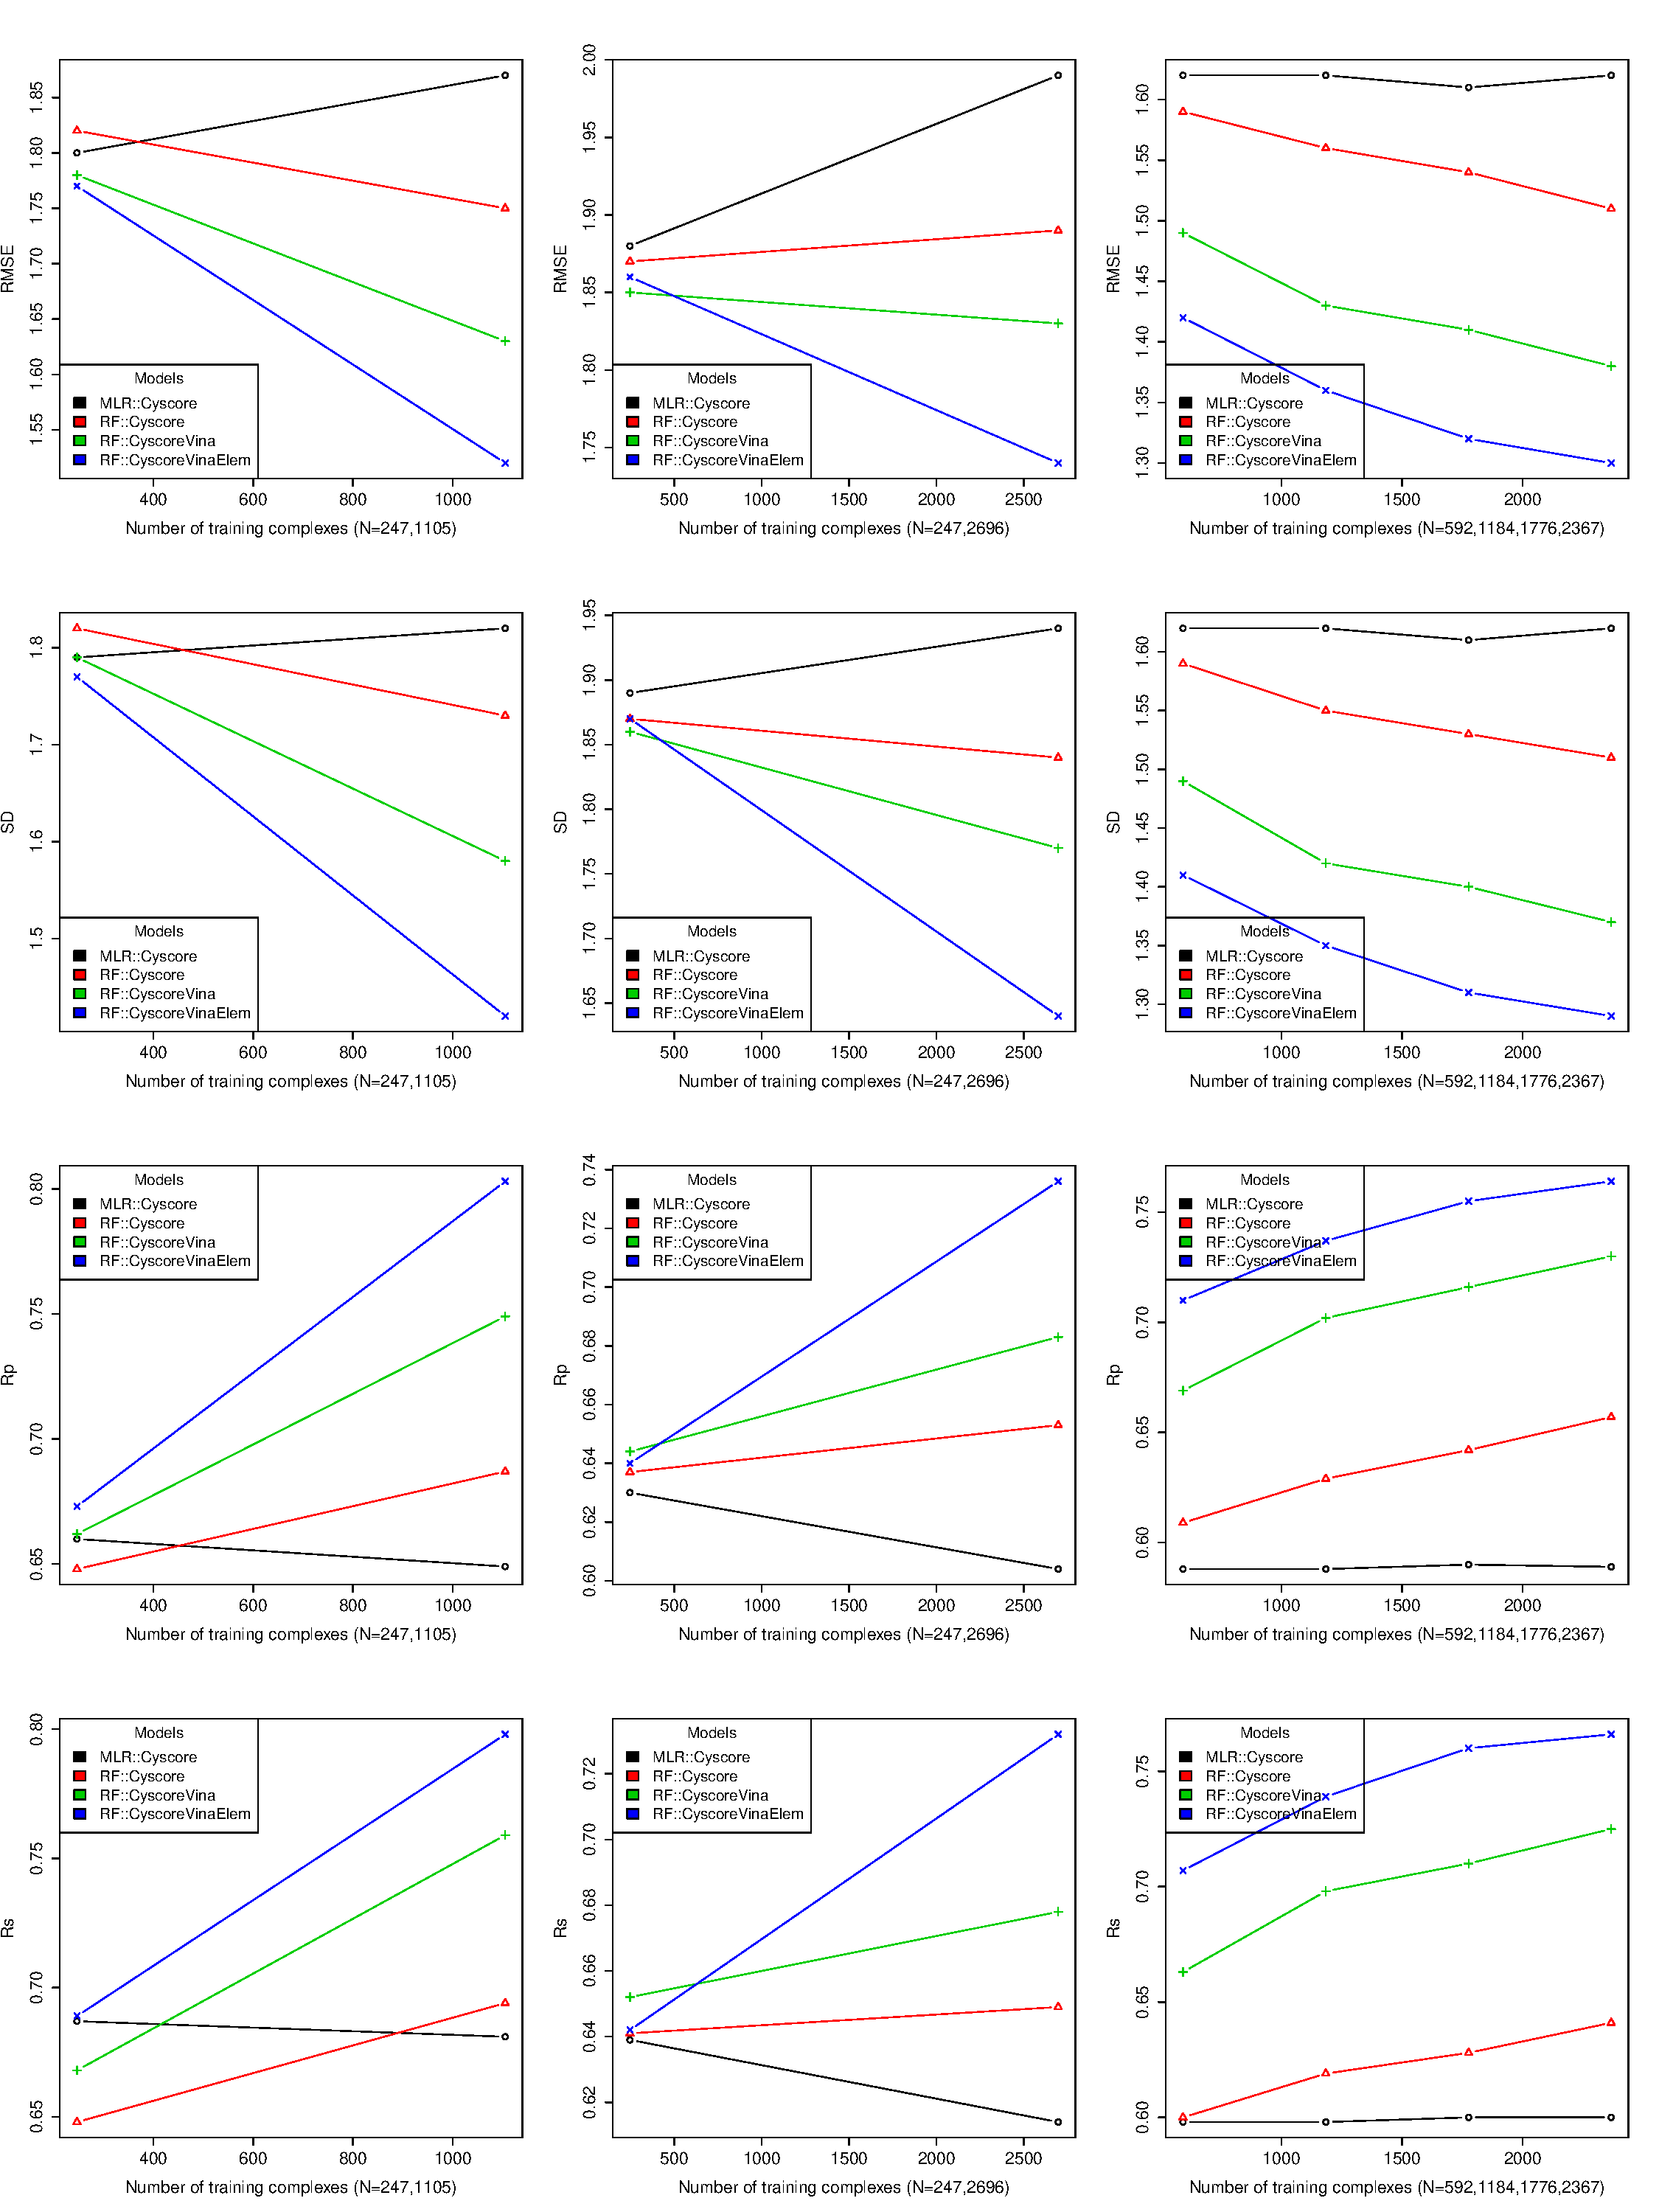
\includegraphics[natwidth=15in,natheight=20in,width=0.98\linewidth]{../rfcyscore/stat.pdf}
\caption{\csentence{Prediction performance of MLR::Cyscore, RF::Cyscore, RF::CyscoreVina and RF::CyscoreVinaElem trained with varying numbers of samples.} First row: root mean square error RMSE. Second row: standard deviation SD in linear correlation. Third row: Pearson correlation coefficient Rp. Fourth row: Spearman correlation coefficient Rs. Left column: PDBbind v2007 benchmark (N=195). Center column: PDBbind v2012 benchmark (N=201). Right column: PDBbind v2013 round-robin benchmark (N=592).}
\label{fig:stat}
\end{figure}

%%%%%%%%%%%%%%%%%%%%%%%%%%%%%%%%%%%
%%                               %%
%% Tables                        %%
%%                               %%
%%%%%%%%%%%%%%%%%%%%%%%%%%%%%%%%%%%

%% Use of \listoftables is discouraged.
%%
\section*{Tables}

\begin{table}[ht]
\caption{The statistics of the five partitions of PDBbind v2013 refined set (N=2959).}
\label{tbl:partitions}
\begin{tabular}{rrrr}
\hline
\# & complexes & lowest pKd & highest pKd\\
\hline
1 & 592 & 2.00 & 11.74\\
2 & 592 & 2.00 & 11.80\\
3 & 592 & 2.00 & 11.85\\
4 & 592 & 2.00 & 11.92\\
5 & 591 & 2.05 & 11.72\\
\hline
\end{tabular}
\end{table}

%%%%%%%%%%%%%%%%%%%%%%%%%%%%%%%%%%%
%%                               %%
%% Additional Files              %%
%%                               %%
%%%%%%%%%%%%%%%%%%%%%%%%%%%%%%%%%%%

\section*{Additional Files}

\subsection*{cv.csv}
This CSV file contains the PDB IDs and measured binding affinities of the protein-ligand complexes in the five partitions of PDBbind v2013 refined set for cross validation purpose.

\end{backmatter}
\end{document}
